%% This is file `elsarticle-template-1-num.tex',
%%
%% Copyright 2009 Elsevier Ltd
%%
%% This file is part of the 'Elsarticle Bundle'.
%% ---------------------------------------------
%%
%% It may be distributed under the conditions of the LaTeX Project Public
%% License, either version 1.2 of this license or (at your option) any
%% later version.  The latest version of this license is in
%%    http://www.latex-project.org/lppl.txt
%% and version 1.2 or later is part of all distributions of LaTeX
%% version 1999/12/01 or later.
%%
%% The list of all files belonging to the 'Elsarticle Bundle' is
%% given in the file `manifest.txt'.
%%
%% Template article for Elsevier's document class `elsarticle'
%% with numbered style bibliographic references
%%
%% $Id: elsarticle-template-1-num.tex 149 2009-10-08 05:01:15Z rishi $
%% $URL: http://lenova.river-valley.com/svn/elsbst/trunk/elsarticle-template-1-num.tex $
%%
\documentclass[preprint,12pt]{elsarticle}

%% Use the option review to obtain double line spacing
%% \documentclass[preprint,review,12pt]{elsarticle}

%% Use the options 1p,twocolumn; 3p; 3p,twocolumn; 5p; or 5p,twocolumn
%% for a journal layout:
%% \documentclass[final,1p,times]{elsarticle}
%% \documentclass[final,1p,times,twocolumn]{elsarticle}
%% \documentclass[final,3p,times]{elsarticle}
%% \documentclass[final,3p,times,twocolumn]{elsarticle}
%% \documentclass[final,5p,times]{elsarticle}
%% \documentclass[final,5p,times,twocolumn]{elsarticle}

%% if you use PostScript figures in your article
%% use the graphics package for simple commands
\usepackage{graphics}
%% or use the graphicx package for more complicated commands
\usepackage{graphicx}
%% or use the epsfig package if you prefer to use the old commands
%% \usepackage{epsfig}

%% The amssymb package provides various useful mathematical symbols
\usepackage{amssymb}
%% The amsthm package provides extended theorem environments
%% \usepackage{amsthm}

%% The lineno packages adds line numbers. Start line numbering with
%% \begin{linenumbers}, end it with \end{linenumbers}. Or switch it on
%% for the whole article with \linenumbers after \end{frontmatter}.
%% \usepackage{lineno}

%% natbib.sty is loaded by default. However, natbib options can be
%% provided with \biboptions{...} command. Following options are
%% valid:

%%   round  -  round parentheses are used (default)
%%   square -  square brackets are used   [option]
%%   curly  -  curly braces are used      {option}
%%   angle  -  angle brackets are used    <option>
%%   semicolon  -  multiple citations separated by semi-colon
%%   colon  - same as semicolon, an earlier confusion
%%   comma  -  separated by comma
%%   numbers-  selects numerical citations
%%   super  -  numerical citations as superscripts
%%   sort   -  sorts multiple citations according to order in ref. list
%%   sort&compress   -  like sort, but also compresses numerical citations
%%   compress - compresses without sorting
%%
%% \biboptions{comma,round}

% \biboptions{}

\usepackage{float}
\usepackage{color}
%%\usepackage{multirow}

\journal{Nuclear Physics B}

\begin{document}

\begin{frontmatter}

%% Title, authors and addresses

%% use the tnoteref command within \title for footnotes;
%% use the tnotetext command for the associated footnote;
%% use the fnref command within \author or \address for footnotes;
%% use the fntext command for the associated footnote;
%% use the corref command within \author for corresponding author footnotes;
%% use the cortext command for the associated footnote;
%% use the ead command for the email address,
%% and the form \ead[url] for the home page:
%%
%% \title{Title\tnoteref{label1}}
%% \tnotetext[label1]{}
%% \author{Name\corref{cor1}\fnref{label2}}
%% \ead{email address}
%% \ead[url]{home page}
%% \fntext[label2]{}
%% \cortext[cor1]{}
%% \address{Address\fnref{label3}}
%% \fntext[label3]{}

\title{Fluorescence Emission Study on Plastic Scintillator EJ-200 After Irradiation}

%% use optional labels to link authors explicitly to addresses:
%% \author[label1,label2]{<author name>}
%% \address[label1]{<address>}
%% \address[label2]{<address>}

\author[umd]{Alberto Belloni}
\author[umd]{Sarah Eno}
\author[umd]{Yongbin Feng}
\author[eljen]{Charles Hurlbut}
\author[umd]{Aaron Hunt}
\author[umd]{Geng-Yuan Jeng}
\author[umd]{Zachary Thomas}
\author[umd]{Yao Yao}
\author[umd]{Zishuo Yang}

\address[umd]{Department of Physics, University of Maryland, College Park, MD 20740, USA}
\address[eljen]{Eljen Technology, 1300 W. Broadway, Sweetwater, TX 79556, USA}

\begin{abstract}
Fluorescence emission yield versus wavelengths for plastic scintillator EJ-200 of various dopant concentrations is measured, 
before and after irradiation by $\rm {^{60}Co}$ source for various doses and dose rates. 
Dose, dose rate, and temperature effects on dopants during irradiations are investigated.
\end{abstract}

\begin{keyword}
%% keywords here, in the form: keyword \sep keyword
plastic scintillator\sep fluorescence\sep radiation damage\sep spectrophotometer

\end{keyword}

\end{frontmatter}

%%
%% Start line numbering here if you want
%%
%%\linenumbers

%% main text
\section{Introduction (to add more)}
Organic plastic scintillators made of polystyrene (PS) or polyvinyltoluene (PVT) substrate and wavelength-shifting dopants have 
long been popular in detectors used in particle physics, nuclear physics, radiation safety, and health physics applications 
due to their high light output, low cost, fast response, and versatility of physical construction. 
Prolonged exposure of plastic scintillator to ionizing radiation, however, can result in damage such that
absorption in the substrate increases and the transfer efficiency from initial excitation of the substrate to the dopants
combined with a dopant's probability of radiative relaxation lessens. 
In this paper, we present fluorescence yield measurements before and after gamma irradiation of various doses and 
dose rates, for one type of plastic scintillator manufactured by Eljen Technology, EJ-200 (similar to BC-408 from Bicron) 
with different concentrations of the primary and secondary dopant.
Dose rate effects are of interest because material-testing is typically done at much higher dose rates than 
which the scintillator will experience in use, due to reactor-time cost.
Dose rate effects may be responsible for the factor-of-three-larger light loss with integrated luminosity 
in the Compact Muon Solenoid (CMS) endcap hadron calorimeter (to cite) than expected based on high dose rate exposure 
using $\rm {^{60}Co}$ sources (to cite). 

The effect of dose and dose rate on radiation-induced absorption increase have been the subject of many investigations (to cite).
The presence of oxygen plays an important role during and after irradiation (to cite).
The studies show that the penetration depth of oxygen into the substrate depends on the dose rate: 
at lower dose rates, oxygen penetrates more deeply (to cite). 
Because of the importance of the interaction of oxygen with radicals produced from the substrate during irradiation, 
this can lead to dose rate effects. Two types of interactions occur in this process. 
The presence of oxygen increases the number of migration mechanisms for the radicals produced during irradiation. 
This allows the radicals that can create color centers which absorbs light to migrate, find other radicals, 
and reform chemical bonds that do not create color centers.
However, as discussed in (to cite Bross), Oxygen also interacts with the radicals produced during irradiation in a way 
that forms color centers. 

Studies on the radiation damage effect on the light yield are fewer than those on the absorption. 
Several studies indicate that damage is to the substrate or the transfer of substrate's emission to dopants, 
rather than on the dopants themselves.
Some studies have indicated that while oxygen plays a beneficial role in regards to annealing of induced absorption effects after 
irradiation, it plays a detrimental role in regards to light output (to cite). 

In order to understand the relative role of destruction of the dopants versus damage to the substrate for modern plastic scintillators, 
we have studied the light output for plastic scintillator EJ-200 with various dopant concentrations, 
for different total doses and dose rates. 

\section{Sample and Irradiation}
EJ-200 uses PVT as a substrate. It has a light output that is 60\% of anthracene and a maximum-emission wavelength of 425 nm (blue). 
Eljen Technology prepared the samples with dimensions of 1x1x5 cm$^{3}$. 
The samples were made with concentration of the primary and secondary dopants at 1.0 and 2.0 that of 
the nominal concentration (which has optimized light output before irradiation). 
1P and 2P refer to nominal and double the nominal concentration of the primary, 
while 1X and 2X refer to nominal and double the nominal concentration of the secondary.
The samples for irradiation were wrapped in Tyvek sheets and were in contact with air.
Using the LHC beamline irradiation facility (CASTOR) at CERN, 
one 1X and one 2X sample were irradiated at about 0.24 krad/hr for a total dose of 0.24 Mrad. (to add uncertainties) 
Using a $\rm {^{60}Co}$ source at the National Institute of Standard and Technology (NIST), some 1P and 2P samples were irradiated  
at rates of 10 krad/hr and 429 krad/hr for a total dose of 3 Mrad, at about 23 $^\circ$C ambient temperature.  
Using a $\rm {^{60}Co}$ source at NASA, one 1P and one 2P sample were irradiated  
at 10 krad/hr for a total dose of 4 Mrad, at about 23 $^\circ$C ambient temperature; 
Two samples that previously received 3 Mrad at 10 krad/hr at NIST were irradiated again at 10 krad/hr for an additional dose of 4 Mrad;
Two 1X samples were irradiated at 80 krad/hr for 5.8 Mrad, at different temperatures 23 $^\circ$C and -30 $^\circ$C.
Additional samples that were produced in the same batch were kept non-irradiated for calibration and comparison.
Table~\ref{table:samples} summarizes the samples irradiated in this study.

\begin{table}[!ht]
\centering
  \caption{Summary of irradiated EJ-200 samples. 
1P and 2P refer to nominal and double the nominal concentration of the primary dopant, 
while 1X and 2X refer to nominal and double the nominal concentration of the secondary dopant.}
  \begin{tabular}{c|c|c}
    \hline
    Dopant concentration 	    & Dose (Mrad)  		& Dose rate (krad/hr)    \\ \hline 
    1P     	    		    & 3 $\pm$  			& 10 $\pm$  	   	 \\ 
    2P     	    		    & 3 $\pm$  			& 10 $\pm$  	   	 \\ \hline
    1P				    & 3 $\pm$			& 429 $\pm$		 \\ 
    2P				    & 3 $\pm$			& 429 $\pm$		 \\ \hline
    1P     	    		    & 4 $\pm$  			& 10 $\pm$  	   	 \\ 
    2P     	    		    & 4 $\pm$  			& 10 $\pm$  	   	 \\ \hline
    1P				    & 7 $\pm$			& 10 $\pm$		 \\ 
    2P				    & 7 $\pm$			& 10 $\pm$		 \\ \hline
    1X     	    		    & 0.24 $\pm$  		& 0.24 $\pm$  	   	 \\ 
    2X     	    		    & 0.24 $\pm$  		& 0.24 $\pm$  	   	 \\ \hline
    1X at ~23 $^\circ$C		    & 6 $\pm$			& 80 $\pm$		 \\ 
    1X at -30 $^\circ$C		    & 6 $\pm$			& 80 $\pm$		 \\
    \hline
  \end{tabular}
  \label{table:samples}
\end{table}

\section{Instrumentation and Techniques}
The fluorescence emission spectra were measured using a FluoroMax-Plus fluorescence spectrometer by Horiba Scientific. 
The spectrometer uses a Xenon arc lamp as continuous light source. 
Light from the lamp is collected by a diamond-turned elliptical mirror and focused on the entrance slit of the excitation monochromator. 
The entrance and exit slits of the excitation monochromator are continuously adjustable, 
which controls the bandpass of the excitation beam. 
A toroidal mirror focuses the excitation beam onto the sample, while a small amount of the beam is split off by a beam-splitter 
to the reference silicon photodiode. 
Fluorescence emission produced by the sample is subsequently collected at ninety-degree angle with respect to the excitation beam. 
Similar to the excitation monochromator, the emission monochromator selects the bandpass of emission light that is sent to 
a Hamamatsu R928 photomultiplier tube (PMT). 
After correcting signals of the PMT and the photodiode according to their quantum efficiencies, 
the fluorescence emission signal is calculated as the ratio of the PMT's signal over the photodiode's signal. 
For each fluorescence spectrum measurement, a fixed excitation wavelength is used, 
and the emission intensity at a range of wavelengths is measured. 

In order to study the effect of radiation damage on the primary and secondary dopants, three excitation wavelengths were chosen: 
285 nm 	exciting PVT and the primary dopant, 
350 nm exciting the secondary and primary dopants, 
and 400 nm exciting mostly the secondary dopant. 
The sample placement in the spectrometer adopts the front-surface configuration (shown in Figure~\ref{fig:sample_placement}), 
which gives the excitation beam a sixty-degree incident angle and maximizes fluorescence emission at the surface. 
This minimizes the effect of self absorption when measuring fluorescence yield after irradiation. 

\begin{figure}[!h]
	\centering
	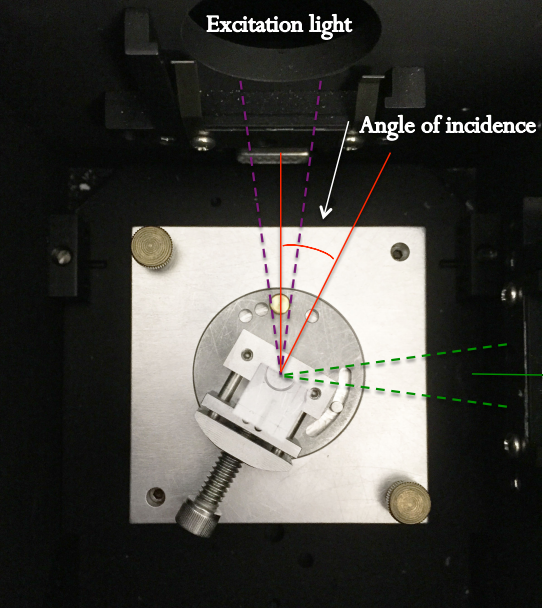
\includegraphics[width=200pt]{./figures/sample_placement.png}
	\caption{Front-surface configuration for fluorescence spectrum measurements.}
	\label{fig:sample_placement}
\end{figure}

\section{Measurements} 
After irradiations, the samples showed coloration which partially disappeared after time due to the annealing of the substrate. 
The samples were repeatedly measured after irradiation until no additional annealing was shown. 
Typical fluorescence spectra of EJ-200 is shown in Figure~\ref{fig:EJ200SP-1P-exc285}, 
after 3 Mrad at 10 krad/hr and after 3 Mrad at 429 krad/hr.

\begin{figure}[!htb]
	\centering
	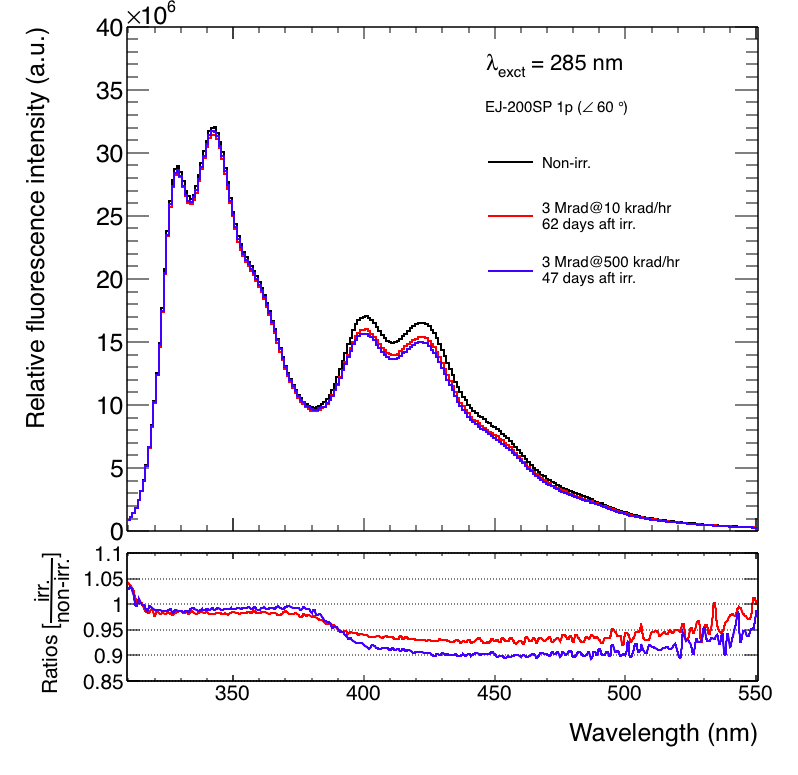
\includegraphics[width=300pt]{./figures/EJ200SP-1P-exc285.png}
	%%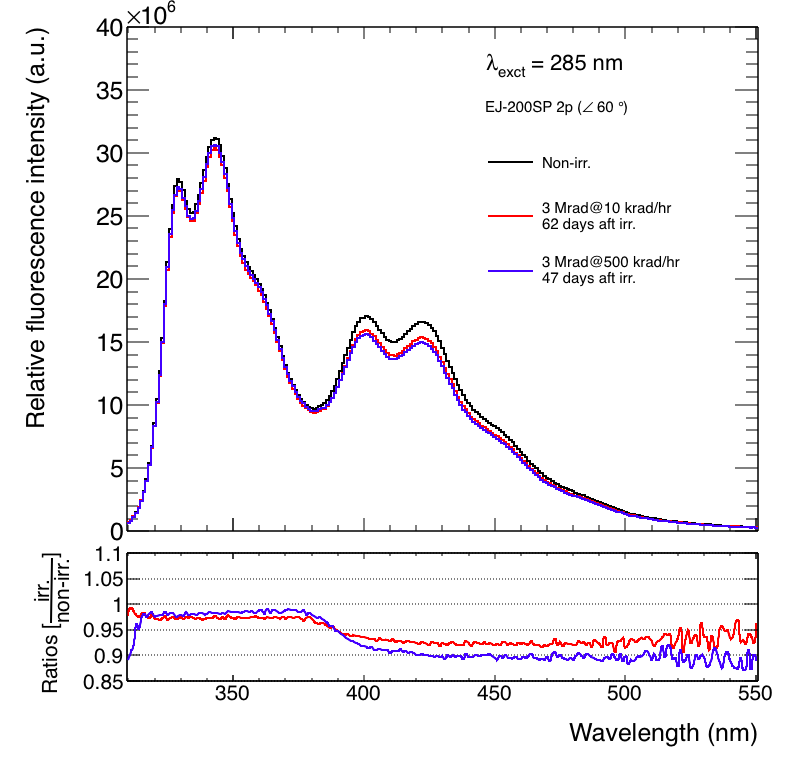
\includegraphics[width=175pt]{./figures/EJ200SP-2P-exc285.png}
	\caption{Fluorescence spectrum excited at 285 nm.}
	\label{fig:EJ200SP-1P-exc285}
\end{figure}

We calculate the light yield ratio (R) using the integrated area of the irradiated sample's spectrum 
with respect to the corresponding non-irradiated one. 

Table~\ref{table:1} shows the ratio of light output excited at three different wavelengths for 
1P {\color{red}{(1P1X?)}} samples of different doses and dose rates. 
Table~\ref{table:2} shows the ratio of light output excited at three different wavelengths for 
1P {\color{red}{(1P1X?)}} samples of different doses at dose rate 10 krad/hr. 
Table~\ref{table:3} shows the ratio of light output excited at three different wavelengths for 
1X {\color{red}{(1P1X?)}} samples of same dose (5.8 Mrad) and dose rate (80 krad/hr), 
but at two different ambient temperatures (23 $^\circ$C and -30 $^\circ$C) during irradiation. 

({\color{red}{Or should I present all the data in one table?}}) 
Table~\ref{table:light-yield-ratio} shows ratio of light output at different excitation wavelengths ($R_{x~nm}$) 
for all the irradiated samples in this study.

\begin{table}[!ht]
\centering
  \caption{Light output ratio after irradiations of different doses and dose rates.}
  \begin{tabular}{l|l|l|l|l}
    \hline
    Dose (Mrad)  & Dose rate (krad/hr)& R at 285 nm	& R at 350 nm	& R at 400 nm    \\ \hline 
    0.24$\pm$    & 0.24$\pm$ 	      & 0.94$\pm$	& 0.94$\pm$	& 0.89$\pm$   \\ \hline
    3.0 $\pm$    & 10 $\pm$	      & 0.95$\pm$	& 0.95$\pm$	& 0.92$\pm$   \\ \hline
    3.0 $\pm$    & 430$\pm$	      & 0.95$\pm$	& 0.92$\pm$	& 0.84$\pm$   \\ 
    \hline
  \end{tabular}
  \label{table:1}
\end{table}

\begin{table}[!ht]
\centering
  \caption{Light output ratio after irradiations of different total doses at dose rate 10 krad/hr.}
  \begin{tabular}{l|l|l|l}
    \hline
    Dose (Mrad)  & R at 285 nm	& R at 350 nm	& R at 400 nm    \\ \hline 
    3.0 $\pm$    & 0.95$\pm$	& 0.95$\pm$	& 0.92$\pm$   \\ \hline
    4.0 $\pm$    & 0.94$\pm$	& 0.92$\pm$	& 0.88$\pm$   \\ \hline
    7.0 $\pm$    & 0.91$\pm$	& 0.88$\pm$	& 0.82$\pm$   \\ 
    \hline
  \end{tabular}
  \label{table:2}
\end{table}

\begin{table}[!ht]
\centering
  \caption{Light output ratio after irradiations of the same dose and dose rate at 23 $^\circ$C and -30 $^\circ$C.}
  \begin{tabular}{l|l|l|l}
    \hline
    T ($^\circ$C)  & R at 285 nm	& R at 350 nm	& R at 400 nm    \\ \hline 
    23  $\pm$    & 0.90$\pm$	& 0.88$\pm$	& 0.78$\pm$   \\ \hline
    -30 $\pm$    & 0.91$\pm$	& 0.84$\pm$	& 0.70$\pm$   \\ 
    \hline
  \end{tabular}
  \label{table:3}
\end{table}

\begin{table}[!ht]
\centering
  \caption{Ratio of light output excited at different wavelengths to that before irradiation for EJ-200 scintillators. 
1P and 2P refer to nominal and double the nominal concentration of the primary dopant, 
while 1X and 2X refer to nominal and double the nominal concentration of the secondary dopant.}	
  \begin{tabular}{c|c|c|c|c|c}
    \hline
    Dopant concentration & Dose (Mrad) 	& Dose rate (krad/hr)    &$R_{285~nm}$	&$R_{350~nm}$	&$R_{400~nm}$	\\ \hline
    1P     	    	 & 3 $\pm$  	& 10 $\pm$  	   	 &0.95 $\pm$	&0.95 ${\pm}$	&0.92 ${\pm}$	\\ 
    2P     	    	 & 3 $\pm$  	& 10 $\pm$  	   	 &0.95 ${\pm}$	&0.95 ${\pm}$	&0.92 ${\pm}$	\\ \hline
    1P			 & 3 $\pm$	& 429 $\pm$		 &0.95 ${\pm}$	&0.91 ${\pm}$	&0.84 ${\pm}$	\\ 
    2P			 & 3 $\pm$	& 429 $\pm$		 &0.95 ${\pm}$	&0.91 ${\pm}$	&0.84 ${\pm}$	\\ \hline
    1P     	    	 & 4 $\pm$  	& 10 $\pm$  	   	 &0.93 ${\pm}$	&0.92 ${\pm}$	&0.87 ${\pm}$	\\ 
    2P     	    	 & 4 $\pm$  	& 10 $\pm$  	   	 &0.94 ${\pm}$	&0.93 ${\pm}$	&0.90 ${\pm}$	\\ \hline
    1P			 & 7 $\pm$	& 10 $\pm$		 &0.90 ${\pm}$	&0.88 ${\pm}$	&0.81 ${\pm}$	\\ 
    2P			 & 7 $\pm$	& 10 $\pm$		 &0.90 ${\pm}$	&0.89 ${\pm}$	&0.83 ${\pm}$	\\ \hline
    1X     	    	 & 0.24 $\pm$  	& 0.24 $\pm$  	   	 &0.94 ${\pm}$	&0.94 ${\pm}$	&0.88 ${\pm}$	\\ 
    2X     	    	 & 0.24 $\pm$  	& 0.24 $\pm$  	   	 &0.95 ${\pm}$	&0.97 ${\pm}$	&0.90 ${\pm}$	\\ \hline
    1X at ~23 $^\circ$C	 & 6 $\pm$	& 80 $\pm$		 &0.90 ${\pm}$	&0.88 ${\pm}$	&0.77 ${\pm}$	\\ 
    1X at -30 $^\circ$C	 & 6 $\pm$	& 80 $\pm$		 &0.90 ${\pm}$	&0.84 ${\pm}$	&0.70 ${\pm}$	\\
    \hline
  \end{tabular}
  \label{table:light-yield-ratio}
\end{table}


%% The Appendices part is started with the command \appendix;
%% appendix sections are then done as normal sections
%% \appendix

%% \section{}
%% \label{}

%% References
%%
%% Following citation commands can be used in the body text:
%% Usage of \cite is as follows:
%%   \cite{key}          ==>>  [#]
%%   \cite[chap. 2]{key} ==>>  [#, chap. 2]
%%   \citet{key}         ==>>  Author [#]

%% References with bibTeX database:

\bibliographystyle{model1-num-names}
\bibliography{<your-bib-database>}

%% Authors are advised to submit their bibtex database files. They are
%% requested to list a bibtex style file in the manuscript if they do
%% not want to use model1-num-names.bst.

%% References without bibTeX database:

% \begin{thebibliography}{00}

%% \bibitem must have the following form:
%%   \bibitem{key}...
%%

% \bibitem{}

% \end{thebibliography}


\end{document}

%%
%% End of file `elsarticle-template-1-num.tex'.
